\section{Methoden}
	
	Dieser Abschnitt befasst sich mit dem Aufbau des Versuches und den dabei auftretenden Unsicherheiten.
	
	\subsection{Aufbau}	
		
		\begin{figure}[ht]
			\centering
			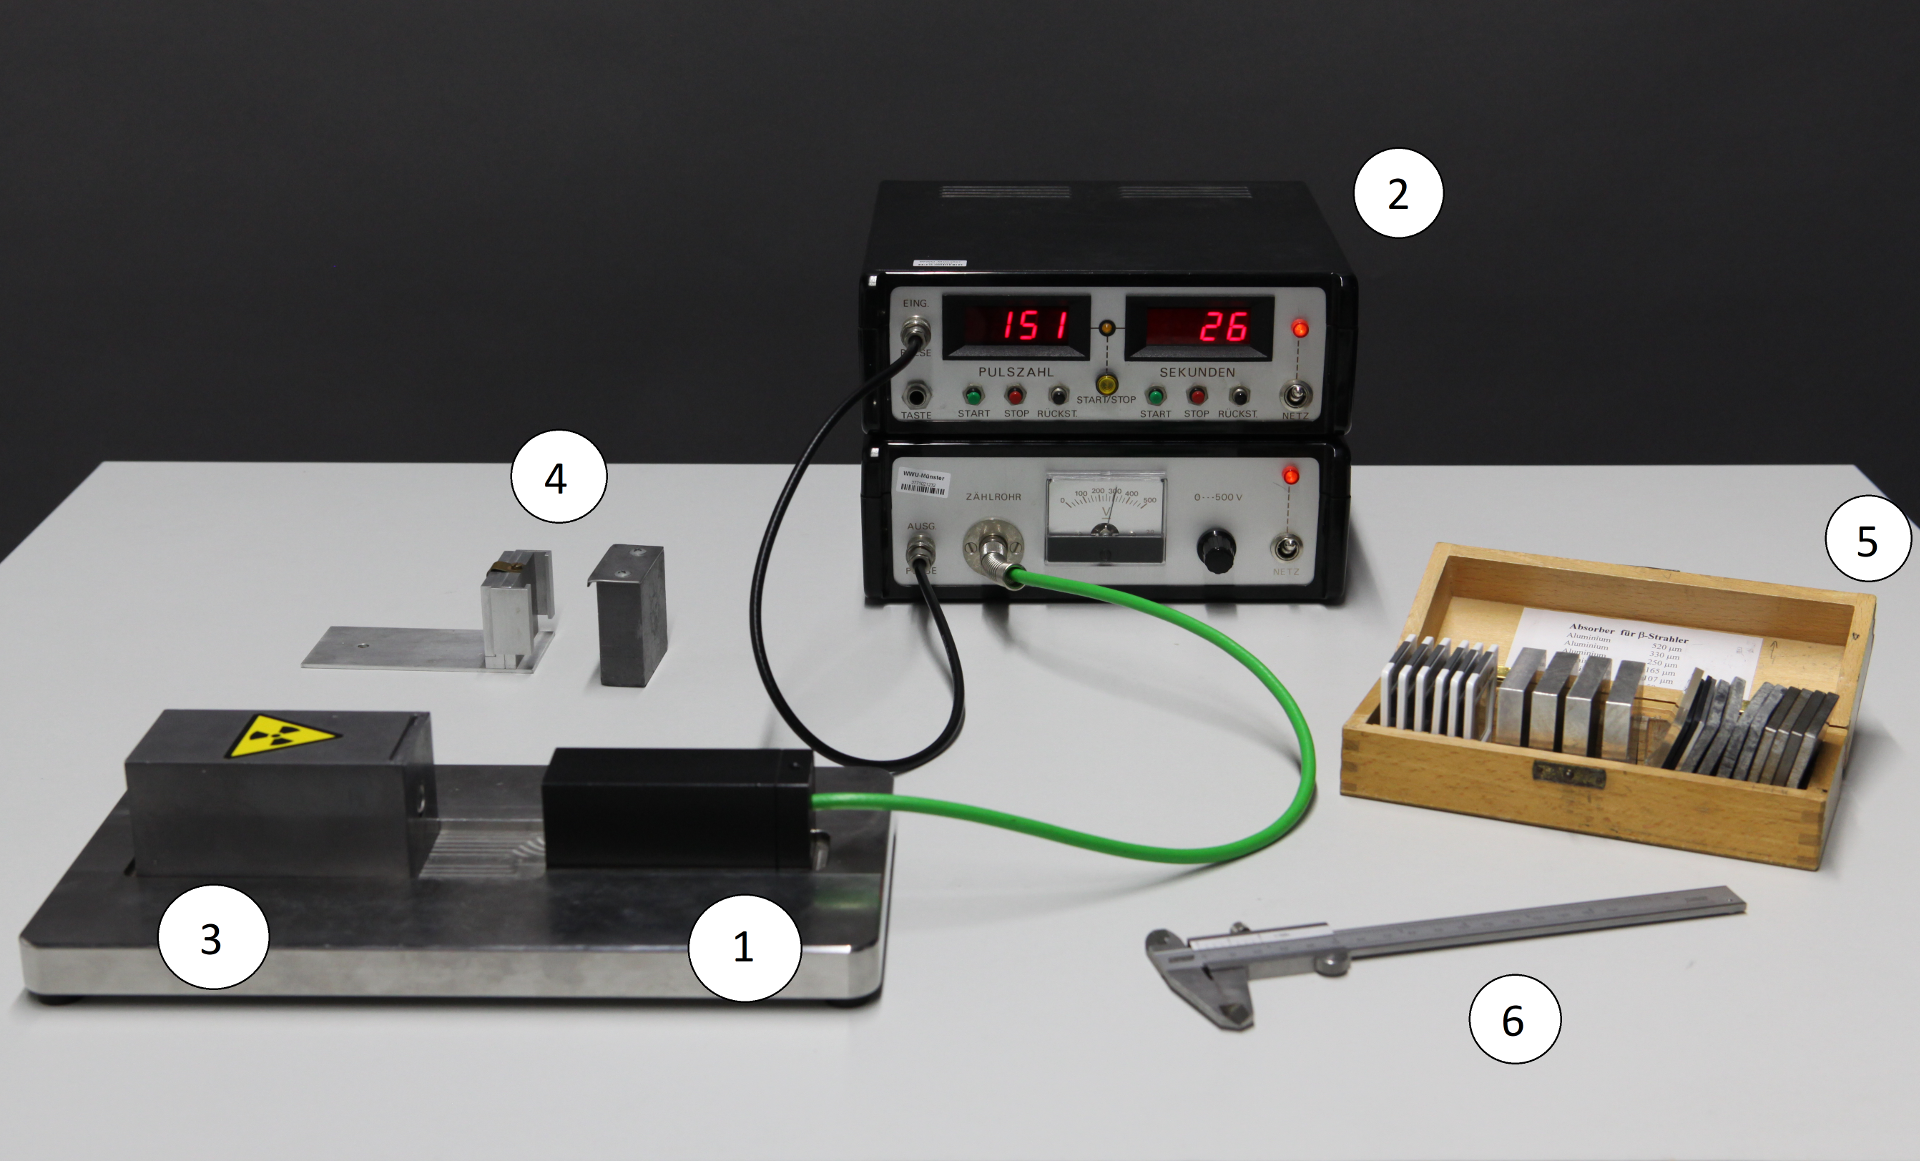
\includegraphics[width=\textwidth]{Aufbau.png}
			\caption{Aufbau des Versuches.\cite{WWU}}
			\label{fig:Aufbau}	
		\end{figure}
		Der Aufbau, wie er in in Abb. \ref{fig:Aufbau} dargestellt ist, besteht im Wesentlichen aus einem Geiger-Müller-Zählrohr (1) mit zugehöriger Messapparatur (2) und einem radioaktiven Präparat, welches in geringem Abstand (wenige Zentimeter) von dem Zählrohr steht.
		Bei den verwendeten radioaktiven Präparaten handelt es sich um den $\beta$-Strahler $^{90}$Sr (4) und den $\gamma$-Strahler $^{137}$Cs (3).
		Zwischen dem Zählrohr und das Präparat können kleine Platten aus Absorbermaterialien (5) platziert werden, sodass eine Messung der Impulsrate in Abhängigkeit der Dicke des Absorbers möglich ist.
		Zur Messung der Dicke der Platten steht eine Schiebelehre (6) zur Verfügung.
		
		Mit Hilfe der Messapparatur die an das Zählrohr geschlossen ist, lassen sich die Anzahl der Impulse bzw. radioaktiven Ereignissen wie auch die vergangene Zeit einfach von einem Digitaldisplay ablesen.
		Zudem lässt sich dort durch einen Drehregler die Betriebsspannung des Zählrohres einstellen.
		
		Zur Messung der natürlichen Strahlung wird das Präparat, welches vor dem Zählrohr platziert ist, entfernt.
				
	\subsection{Unsicherheiten}
	
		Jegliche Unsicherheiten werden nach GUM bestimmt und berechnet\footnote{Die Gleichungen dazu finden sich im Anhang unter \ref{fig:GUM_combine}, \ref{fig:GUM_formula}.}.
		Für die Unsicherheitsrechnungen wurde die Python Bibliothek "uncertainties" herangezogen, welche den Richtlinien des GUM folgt.
	
		Für digitale Messungen wird eine Unsicherheit von $u(X) = \frac{\Delta X}{\sqrt{3}}$ angenommen, bei analogen eine von $u(X) = \frac{\Delta X}{\sqrt{6}}$.
		
		\begin{itemize}
			\item Mit Hilfe des analogen Voltmeters an der Messapparatur konnte die Betriebsspannung mit $\Delta U = \SI{25}{\volt}$ eingestellt werden.
			
			\item Die Zeit wurde mit einem digitalen Sekundenzähler aufgenommen.
			Dadurch ergibt sich $\Delta T = \SI{1}{\second}$.
			
			\item Die Dicken der einzelnen Absorberplatten wurden, soweit möglich, mit einer Schiebelehre nachgemessen.
			Diese hatte eine Unsicherheitsangabe von $\Delta d = \SI{0.05}{\milli\meter}$.
			Die Dicken aller dünnen Aluminiumfolien konnten durch die Schieblehre nicht erfasst werden.
			Für diese wird eine Unsicherheit von $\Delta d = \SI{0.5}{\micro\meter}$ angenommen.
		\end{itemize}
		
\section{Durchführung und Datenanalyse}
		
	Die Zeit bzw. die Zahl der Ereignisse wurde bei allen Messungen so gewählt, dass die relative Unsicherheit unter 4\%, für alle Messwerte liegt.
	Das Wechseln oder Entfernen der radioaktiven Präparate wurde von dem Betreuer durchgeführt.
	
	Zur Bestimmung der Zählrohrcharakteristik wurde der $\beta$-Strahler $^{90}$Sr verwendet und für verschiedene Spannungen die Anzahl der Ereignisse nach \SI{94+-0,2}{\second} aufgetragen. 
	Eine Darstellung der Messwerte ist der Abb. \ref{fig:Kennlinie} zu entnehmen.
	\begin{figure}[ht]
		\centering
		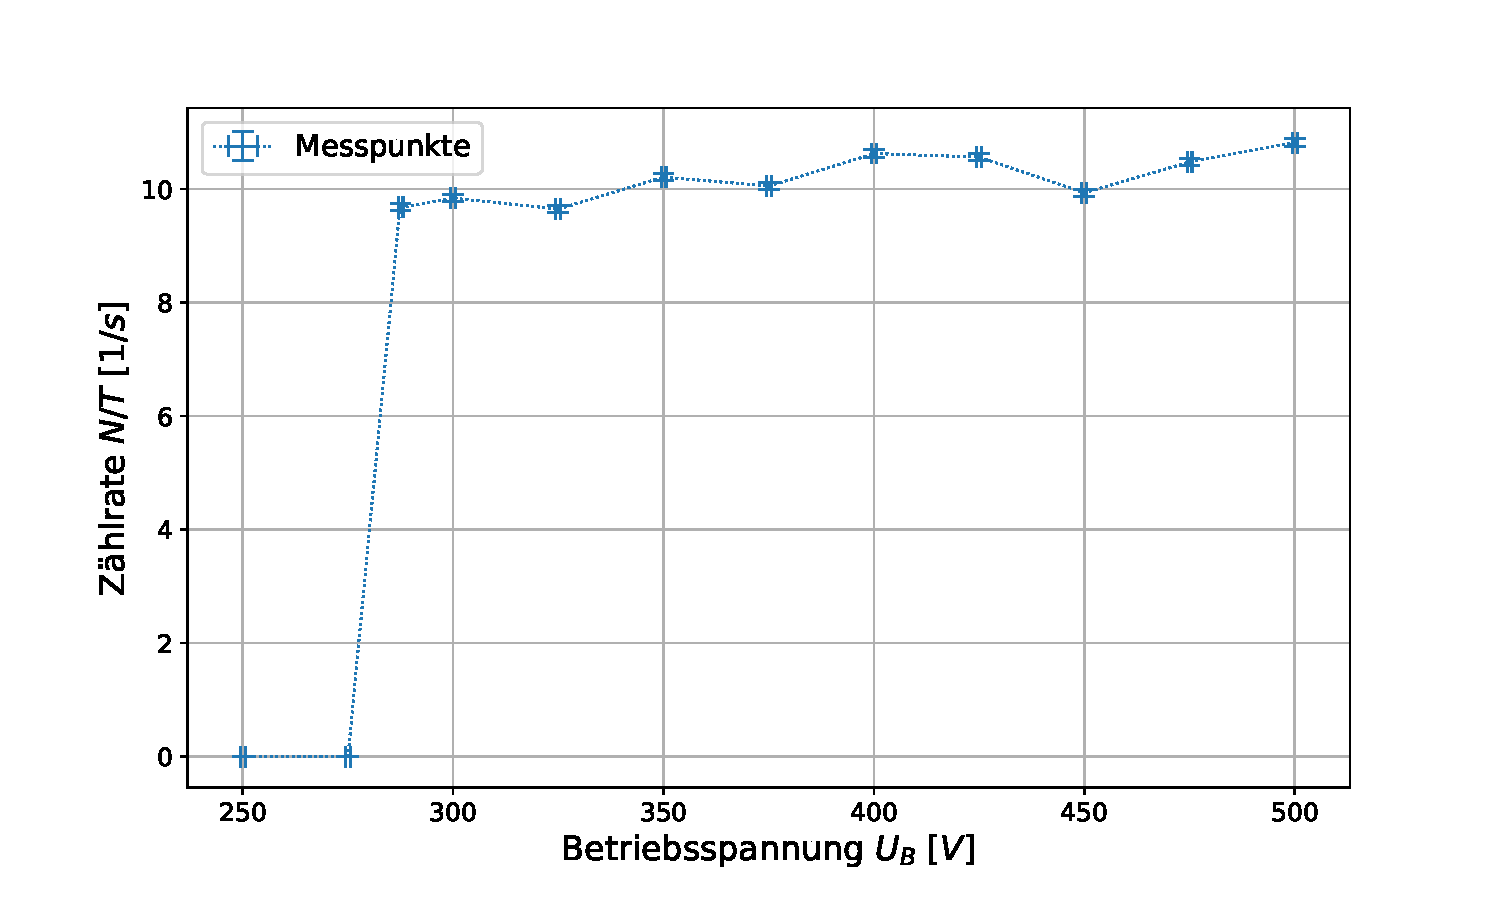
\includegraphics[width=\textwidth]{data/CharakteristikZaehlrohr.pdf}
		\caption{Impulsrate in Abhängigkeit der Spannung am Zählrohr bzw. Zählrohrcharakteristik.}
		\label{fig:Kennlinie}	
	\end{figure}
	Diese Kennlinie zeigt, dass zur Messung der Radioaktivität mindestens eine Spannung von $\approx \SI{275+-7,2}{\volt}$ anliegen muss, diese nennt sich Einsatzspannung. 
	Auch das charakteristische Plateau nach dem Erreichen dieser Spannung ist der Kurve zu entnehmen.
	Zudem ließen sich nur Werte bis zu \SI{500+-7,2}{\volt} einstellen, da höhere Spannungen zur Beschädigung oder gar Zerstörung des Zählrohrs führen könnten. 
	
	Zur Messung der natürlichen Radioaktivität wurde das radioaktive Präparat entfernt und 200 mal die Anzahl der Ereignisse innerhalb von \SI{10}{\second} aufgenommen.
	Aus dieser Verteilung folgen der Mittelwert von $\SI{0.2929+-0.0014}{\becquerel}$ und die empirische Standardabweichung von $\SI{0.1745+-0.0021}{\becquerel}$. 
	\begin{figure}[ht]
		\centering
		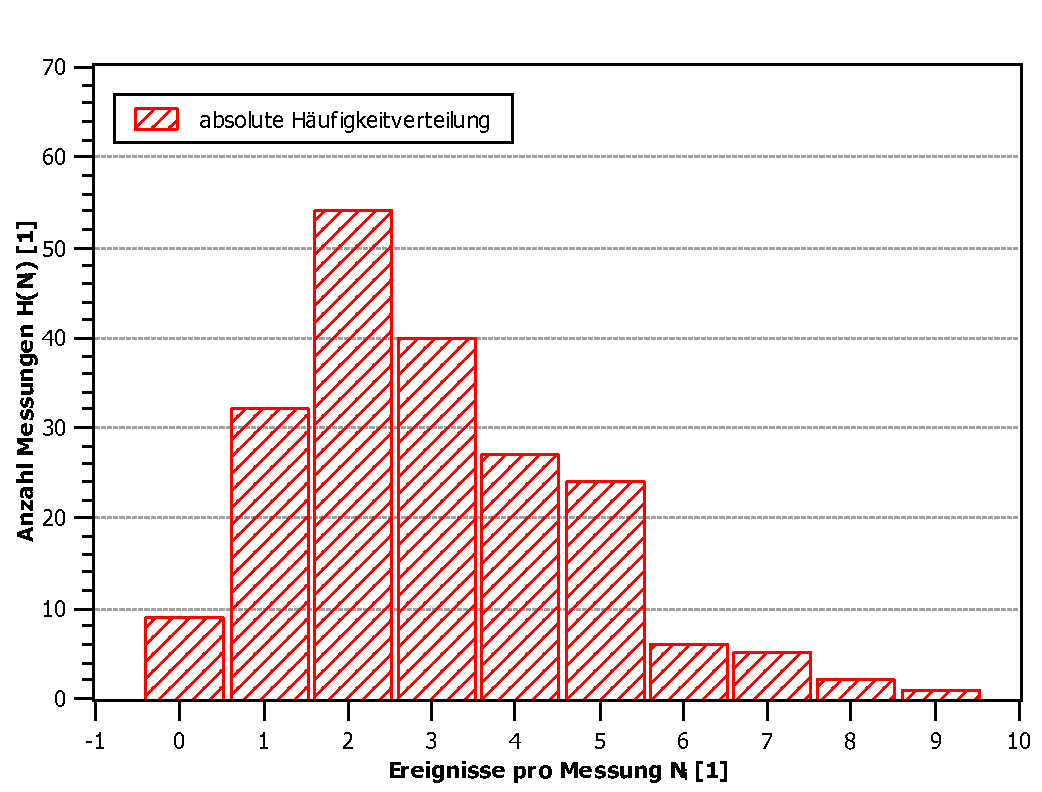
\includegraphics[width=\textwidth]{data/bckgndHistogrammAbs.pdf}
		\caption{Histogramm der absoluten Häufigkeitsverteilung der natürlichen Strahlung.}
		\label{fig:absolut}	
	\end{figure}
	\begin{figure}[ht]
		\centering
		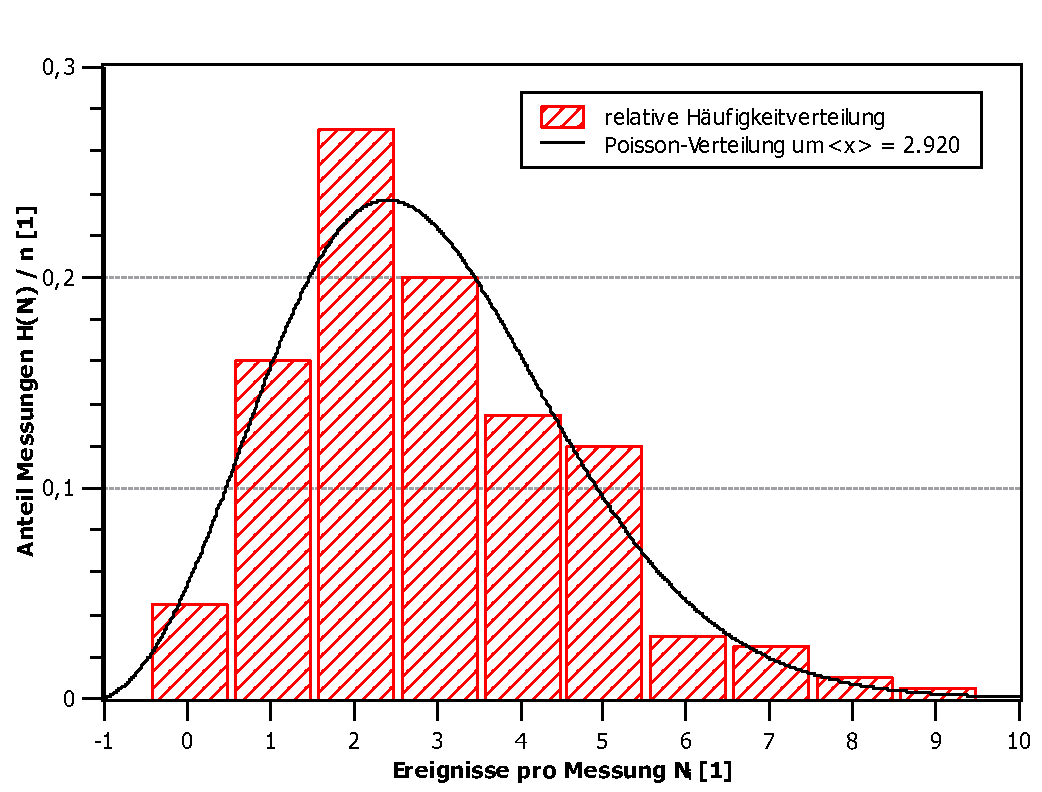
\includegraphics[width=\textwidth]{data/bckgndHistogrammRelPoisson.pdf}
		\caption{Histogramm der relativen Häufigkeitsverteilung der natürlichen Strahlung mit Poisson-Verteilung.}
		\label{fig:relativ}	
	\end{figure}
	Diagramme der absoluten und relativen Häufigkeitsverteilung sind in Abb. \ref{fig:absolut} und Abb. \ref{fig:relativ} vorzufinden. 
	Zur Berechnung der Kurve über der relativen Häufigkeitsverteilung wurde die Poisson-Verteilung herangezogen: 
	\begin{align}
		\psi (N) = \frac{\bar{N}^N\cdot e^{\bar{N}}}{N!}, \quad N = \text{Anzahl der Impulse}, \bar{N} = <N>.
	\end{align} 
	Mit Hilfe der mittleren Untergrundaktivität, die aus der natürlichen Radioaktivität hervorgegangen ist, wurde für die folgenden Messungen eine Korrektur durchgeführt.
	
	Zur Bestimmung des Absorptionskoeffizienten $\mu_\gamma$ von Blei wurde die Impulsrate $a_\gamma (x)$ des $\gamma$-Präparats $^{137}$Cs in Abhängigkeit der Schichtdicke des Blei-Absorbers aufgenommen.	
	Hierbei wurde die Zeit gemessen, die benötigt wurde um ca. 650 Ereignisse in dem Zählrohr auszulösen, um die Impulsrate mit einer relativen Unsicherheit unter 4\% aufzunehmen.
	Zusätzlich wurde die Spannung an dem Zählrohr so gewählt, dass sie mit $\SI{400+-7,2}{\volt}$ ca. \SI{125}{\volt} über der Einsatzspannung, mitten auf dem Plateau der Zählrohrcharakteristik liegt.
	Nach jeder Messreihe wurde eine weitere Platte hinzugefügt und eine neue Reihe gestartet, sodass die Impulsrate in Abhängigkeit der Schichtdicke aufgetragen werden konnte.
	Dazu standen vier Blei-Platten zur Verfügung.
	\begin{figure}[ht]
		\centering
		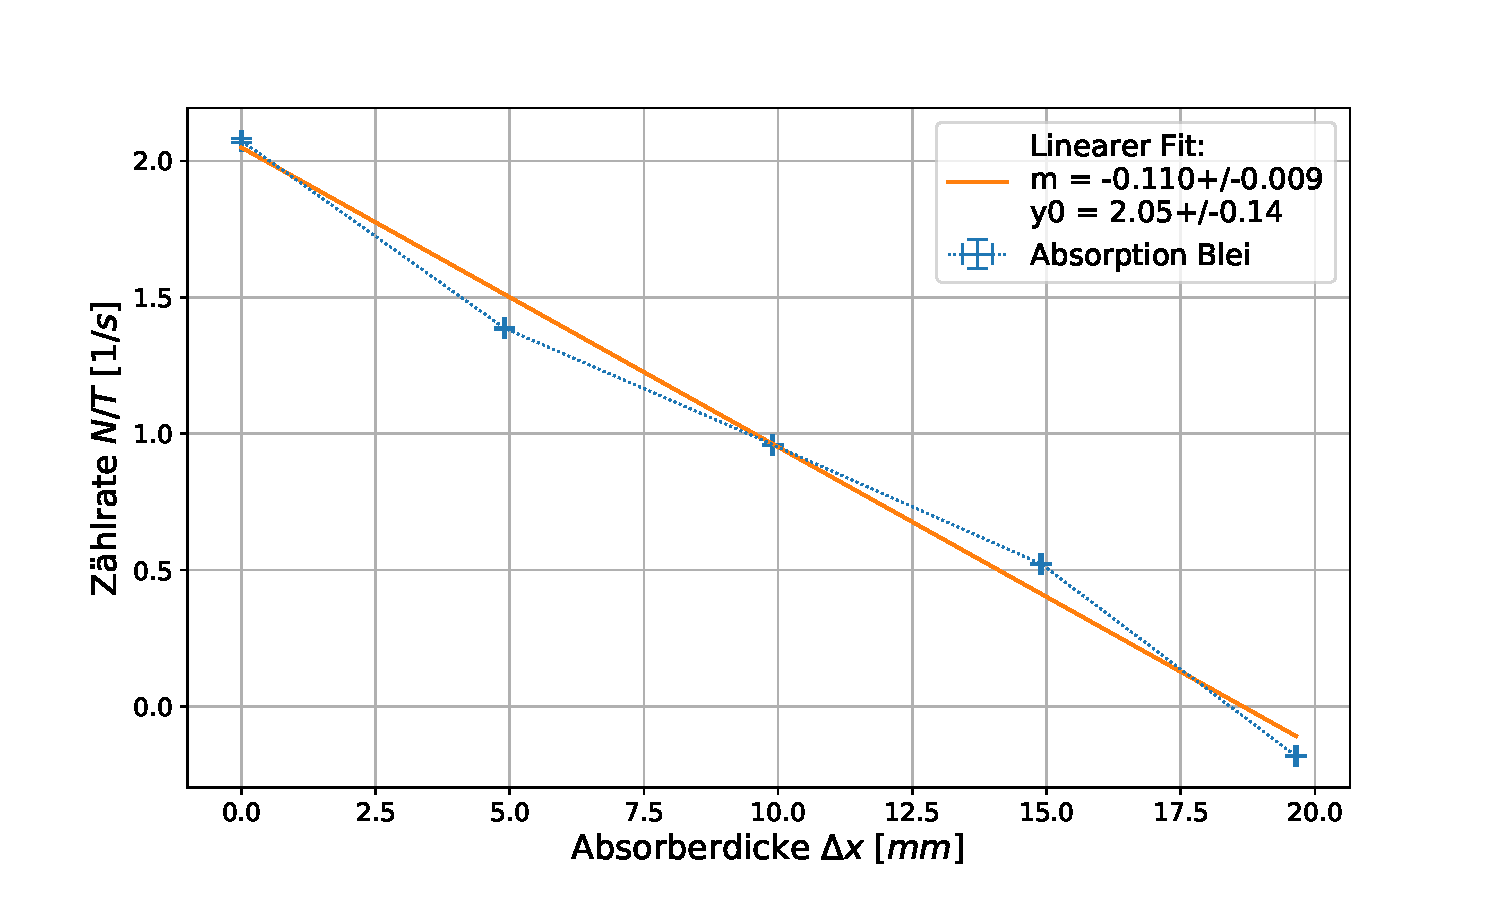
\includegraphics[width=\textwidth]{data/GammaAbsorber.pdf}
		\caption{Impulsrate in Abhängigkeit der Schichtdicke des Bleis. Dabei gilt für die Steigung des Fits $m = -\mu_\gamma$.}
		\label{fig:gamma}	
	\end{figure}
	Abb. \ref{fig:gamma} stellt das Verhältnis logarithmisch aufgetragen dar. 
	Da es sich bei steigender Schichtdicke um einen exponentiellen Abfall der Ereignisse handeln sollte ($N(x) = N_0 e^{-\mu x}$), lässt sich der Absorptionskoeffizient aus der Steigung des Graphen bestimmen.
	Dieser Koeffizient und der Massenabsorptionskoeffizient, der sich durch teilen ersteren durch die Dichte des Bleis ergibt sind in der Tabelle \ref{tab:Werte} aufgeführt.
	
	Analog verlief die Messung der Impulsraten $a_\beta (x)$ des $\beta$-Präparats $^{90}$Sr in Abhängigkeit der Schichtdicken von Aluminium, Plexiglas und Gummi.
	Für die letzteren beiden, wurde die Messung jedoch nur für je eine Schicht durchgeführt.
	\begin{figure}[ht]
		\centering
		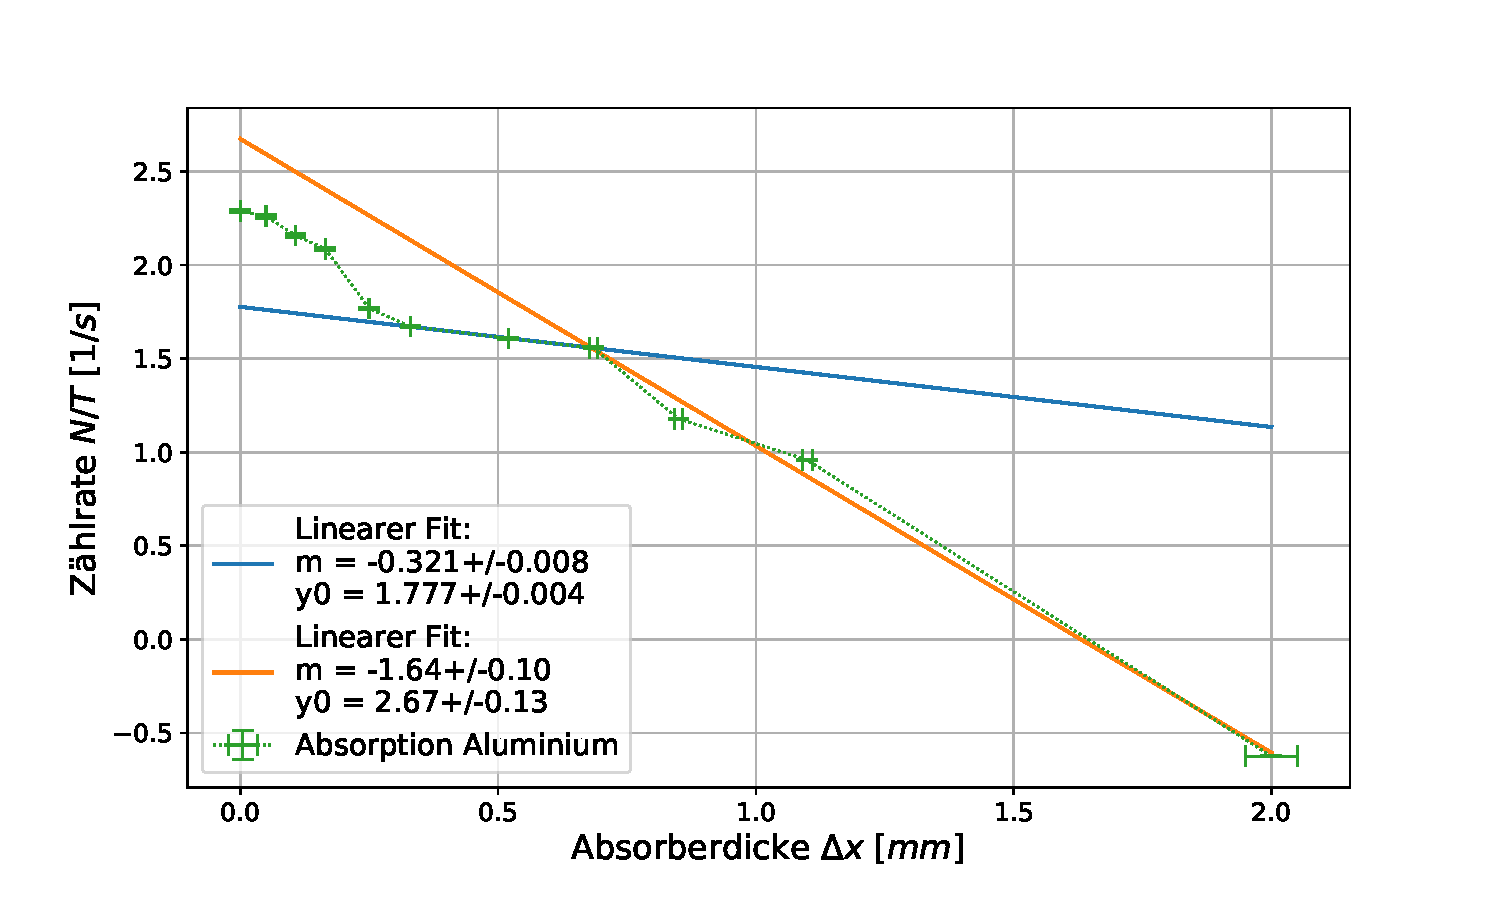
\includegraphics[width=\textwidth]{data/BetaAbsorber.pdf}
		\caption{Impulsrate in Abhängigkeit der Schichtdicken von Aluminium. Hier wurden zwei mögliche Steigungen dargestellt, für die weitere Auswertung wurde jedoch nur die Steigung des orangefarbenen Fits betrachtet.}
		\label{fig:beta}	
	\end{figure}
	\begin{figure}[ht]
		\centering
		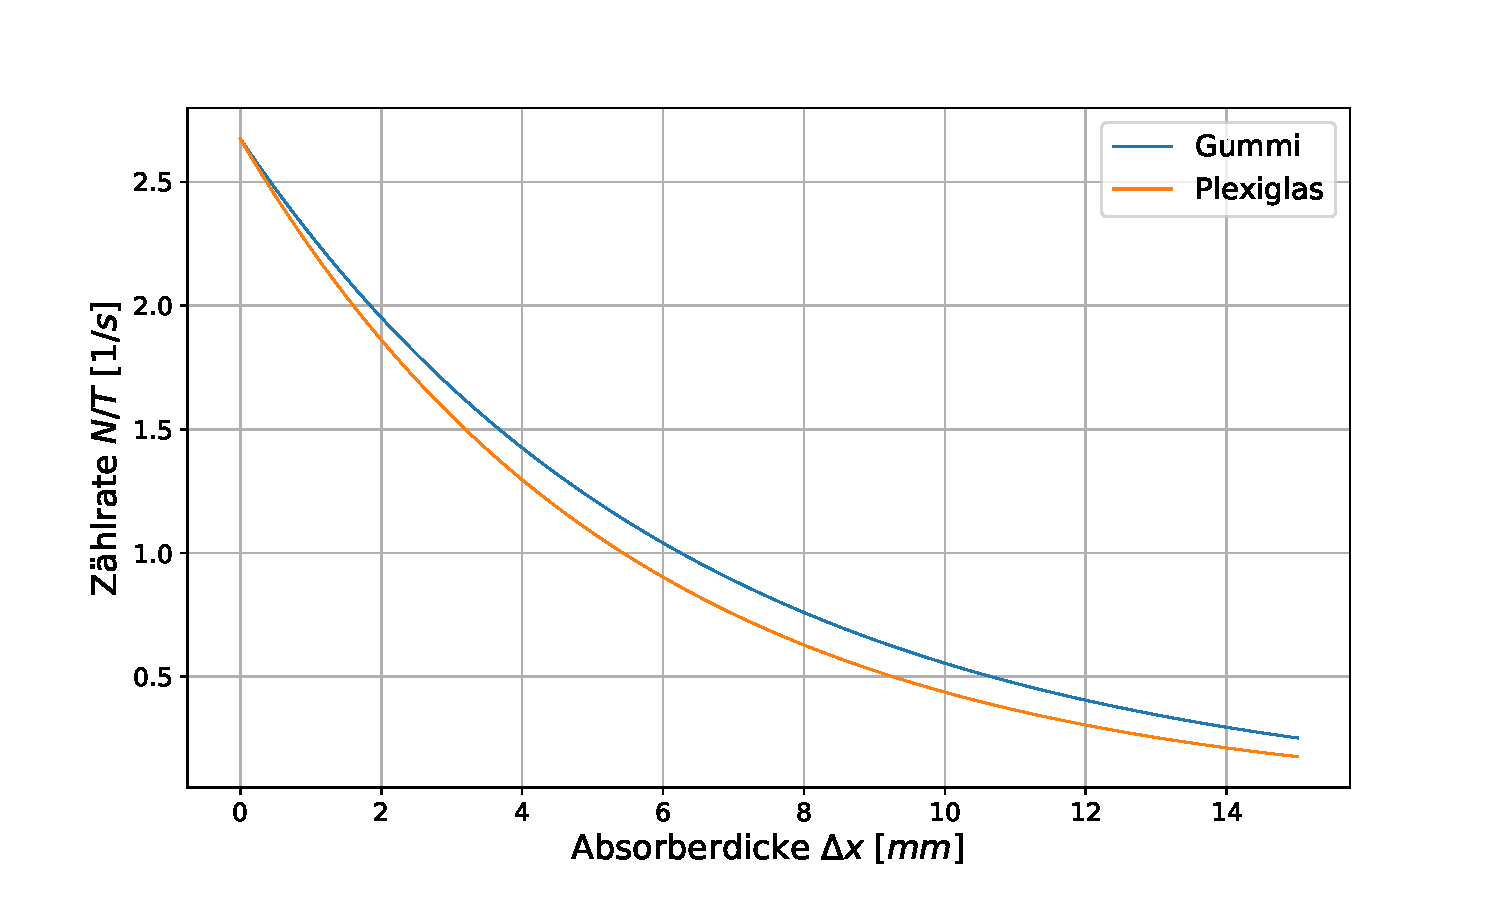
\includegraphics[width=\textwidth]{data/GummiPlexiAbsorber2.pdf}
		\caption{Impulsrate in Abhängigkeit der Schichtdicken von Plexiglas und Gummi.}
		\label{fig:beta2}	
	\end{figure}
	Eine graphische Darstellung der Messung ist in den Abb. \ref{fig:beta} und \ref{fig:beta2} vorzufinden. 
	Die sich dadurch berechneten Koeffizienten sind ebenso in Tab. \ref{tab:Werte} verzeichnet. 
	
	\begin{table}
		\caption{In dieser Tabelle sind die ermittelten Absorptions- und Massenabsorptionskoeffizienten aufgetragen. Zu letzteren sind zusätzlich Literaturwerte angegeben.\cite{NIST}\cite{Tikrit}}
		\label{tab:Werte}
		\centering
		\begin{tabular}{c|c|c|c|c}					
			& Blei ($\mu_\gamma$) & Aluminium ($\mu_\beta$) & Plexiglas ($\mu_\beta$) & Gummi ($\mu_\beta$) \\
			\hline	
			$\mu$ (\si{\per\centi\meter}) & \SI{1.10+-0.09}{} & \SI{16.4+-1.0}{} & \SI{1.81+-0.12}{} & \SI{1.57+-0.25}{} \\
			$\mu_m$ (\si{\centi\meter^2\per\gram}) & \SI{9.7+-0.8e-2}{} & \SI{6.08+-0.35}{} & \SI{1.95+-0.13}{} & \SI{1.69+-0.27}{} \\
			$\mu_{m,Lit}$ (\si{\centi\meter^2\per\gram}) & \SI{8.870e-2}{} & \SI{33,99}{} & &\\
			\hline
			Abweichung & 9,4\% & 82.1\% & &	
		\end{tabular}
	\end{table}
	
\section{Diskussion}
	
	Nun stellt sich die Frage, ob die Ergebnisse dem Ziel dieser Untersuchung genügen.
	
	Wird dazu zunächst die aufgenommene Zählrohrcharakteristik betrachtet, so lässt sich der zu erwartende Verlauf klar in dieser erkennen.
	Bis zur Einsatzspannung werden keine Impulses gemessen und die Werte, welche auf dem Plateau vorzufinden sind, liegen alle auf einer Ebene und weichen nur gering voneinander ab.
	
	Das Histogramm der relativen Häufigkeitsverteilung der natürlichen Strahlung zeigt, dass die Verteilung sich in guter Näherung durch die Poisson-Verteilung bestimmen lässt, da der Verlauf der Poisson-Kurve, um den Mittelwert von 2,92 Impulsen pro zehn Sekunden, das Histogramm nahezu lückenlos einschließt.
	Nur am Erwartungswert selber hebt sich das Histogramm etwas von der Kurve ab, dies ist jedoch zu vernachlässigen.
	
	Vergleicht man nun die Ergebnisse der Absorption, so erkennt man zunächst, dass die Messung der Impulsrate in Abhängigkeit der Schichtdicke des Bleis in etwa mit den Erwartungen übereinstimmt.
	Es ließ sich bei logarithmischer Auftragung der Messwerte eine Gerade mit negativer Steigung durch die Messpunkte legen, was für den exponentiellen Abfall der Impulsrate spricht.
	Der aus dieser Steigung entstehende Absorptionskoeffizient führte durch teilen durch die Dichte des Bleis zu einem Massenabsorptionskoeffizienten, der sich mit der Literatur vergleichen lässt.	
	Bei dem Literaturwert handelt es sich um den, auf dem Energiespektrum der $^137$Cs-$\gamma$-Strahlung, der am stärksten mit dem ermittelten Wert übereinstimmt.
	Der Vergleich zeigt eine Abweichung von 9,4\%, was  in grober Näherung dem Literaturwert entspricht.
	
	Bei dem Aluminium zeigt bereits die Messkurve, dass sich kein "passender" linearer Fit finden konnte.
	Auch der Massenabsorptionskoeffizient der näher an dem Literaturwert liegt, weicht um 82,1\% von diesem ab.
	Hier kann keine Übereinstimmung mit der Literatur gefunden werden, da diese Abweichung zu groß ist.
	
	Für das Plexiglas und Gummi ließen sich keine Literaturwerte finden. 
	Zudem wurden für die Bestimmung der Absorptionskoeffizienten nur je zwei Messpunkte herangezogen.
	Aus diesen lässt sich zumindest erkennen, dass das Plexiglas die $\beta$-Strahlung besser absorbiert als Gummi
	
	Würde Blei als Absorber für die $\beta$-Strahlung gewählt, so wären vermutlich keine Impulse neben denen der natürlichen Strahlung gemessen worden, was aus der Dichte von Blei und der bereits starken Absorption von deutlich mehr durchdringender $\gamma$-Strahlung hervorgeht.
	